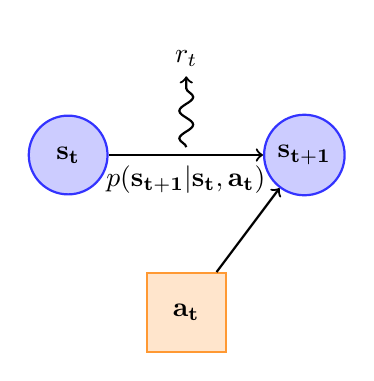
\begin{tikzpicture}
\tikzstyle{state}=[circle,
thick,
minimum size=1.0cm,
draw=blue!80,
fill=blue!20]
\tikzstyle{action}=[rectangle,thick,
minimum size=1.0cm,
draw=orange!80,
fill=orange!20]

  \node[state] (st) at (0,0) {$\mathbf{s_t}$};
  \node[action] (at) at (1.5,-2) {$\mathbf{a_{t}}$};
  \node[state] (stpu) at (3,0) {$\mathbf{s_{t+1}}$};
  \draw[->,thick] (at) --  (stpu);
  \draw[->,thick] (st) -- node[below] {$p(\mathbf{s_{t+1}}|\mathbf{s_t},\mathbf{a_t})$}(stpu);
  \draw[->,thick,decorate,decoration={snake}] (1.5,0.1) -- (1.5,1);
  \node[anchor=south] at (1.5,1.0) {$r_t$};
  \node at (0,1.5) {};
\end{tikzpicture}
